\chapter{Implementacja}
\label{chap:project implementation}
Implementację aplikacji można podzielić na frontend zaimplementowany w Next.js obejmujący pobieranie informacji od użytkownika i wyświetlanie wyników działania aplikacji w przystępny sposób oraz backend oparty o język programowania Python i blibliotekę FastAPI obejmujący wykrycie pól i lasów dla zadanych przez użytkownika punktów oraz zaplanowanie trasy, która zostanie zwrócona użytkownikowi, a także implementację API wykorzystywanego przez frontend aplikacji do kierowania żądań.

\section{Warstwa interakcji z użytkownikiem}

\section{Opis zaimplementowanego API dla frontendu (?)}

\section{Wykrywanie pól i lasów (Wiktoria Kubacka)}
Ta część aplikacji jest odpowiedzialna za przetworzenie podanych przez użytkownika współrzędnych w celu wyodrębnienia obszarów na zdjęciach satelitarnych, na których będzie przebiegała zaplanowana przez aplikację trasa dla bezzałogowego statku powietrznego. Cały proces wykrywania obszarów składa się z przetworzenia podanych przez użytkownika punktów, wykrycia krawędzi pól i lasów na zdjęciach satelitarnych, a następnie wyodrębnienia wykrytych obszarów ze zdjęć. Wynikiem działania tej części aplikacji jest lista punktów, która pozwala na odtworzenie konturu wykrytego obszaru w celu zaplanowania trasy i prezentacji wykrytego obszaru użytkownikowi.

\subsection{Wykorzystanie API oraz zewnętrznych bibliotek}
Aplikacja korzysta z biblioteki Earth Engine pozwalającej na wykorzystanie API Google Earth Engine pozwalającego na dostęp do zdjęć z satelity Sentinel2 oraz szybkiego przetworzenia ich, by wyodrębnić krawędzie obszarów. Ponadto, na przekształcenie uzyskanych krawędzi na obszary i wyodrębnienie z nich punktów pozwoliły biblioteki NumPy, Scikit-image oraz OpenCV.  

\subsection{Wykrycie krawędzi obszarów}
Wykrywanie pól i lasów na zdjęciach satelitarnych rozpoczyna się od przetworzenia podanych przez użytkownika współrzędnych na klasę Point wykorzystywanej przez bibliotekę Earth Engine do reprezentacji punktów. Z podanych współrzędnych jest wyliczany centroid, który jest punktem odniesieniem dla dalszych operacji wykonywanych w programie. Detekcja krawędzi jest wykorzystywana z użyciem klasy EdgeDetector. 

Klasa EdgeDetector przyjmuje listę punktów pod postacią FeatureCollection, środek mapy będący obiektem klasy Pont oraz projekcję mapy, na której operuje klasa, będąca klasą Projection. Poza podawanymi parametrami przyjmowanymi przez konstruktor, w metodzie \_\_init\_\_() zostały zdefiniowane parametry wykorzystywane przez klasę:

\begin{itemize}
    \item time\_periods -- lista definiująca przedziały czasu, dla których pobierane są zdjęcia satelitarne
    \item bands -- kanały, na których operujemy podczas wykrywania krawędzi
    \item thresholds -- lista zawierająca progi (niski i wysoki) dla każdego z kanałów barw
    \item sigmas -- wartości parametru sigma, jakie są brane dla każdego z kanałów barw podczas rozmycia gaussowskiego przygotowującego do wykrywania krawędzi w algorytmie Canniego
    \item distance -- parametr definiujący maksymalną odległość, jaka może dzielić krawędzie, by zostały złączone
    \item scale -- skala mapy brana do wyświetlania rezultatu (? to chyba będzie trzeba usunąć z kodu)
    \item cloud\_filter\_threshold -- wartość definiująca maksymalny stopień zachmurzenia poszukiwanych zdjęć satelitarnych
\end{itemize}

\begin{lstlisting}[language=Python, caption=Metoda \_\_init\_\_() klasy EdgeDetector, style=python_style]
def __init__(
    self, points: ee.FeatureCollection,
    map_center: ee.Geometry.Point,
    projection: ee.Projection
    ):
    self.__time_periods = [
        ['2017-06-01', '2017-09-01'],
        ['2018-06-01', '2018-09-01'],
        ['2019-06-01', '2019-09-01'],
        ['2020-06-01', '2020-09-01'],
        ['2021-06-01', '2021-09-01'],
        ['2022-06-01', '2022-09-01'],
        ['2023-06-01', '2023-09-01'],
        ['2024-06-01', '2024-09-01']]  
        # more time periods can provide more accurate data, 
        # but also makes calculations slower
    self.__bands = ['B4', 'B3', 'B2']  
    # bands of satellite imagery that are used for edge detection
    self.__thresholds = [110 if i % 2 == 0 else 120 for i in range(6)]  
    # low and high threshold that is used for each band 
    # [low_band1, high_band1, ... ]
    self.__sigmas = [5, 11, 4]  
    # values of sigma that are used for each of the bands
    self.__distance = 5  
    # max distance between edges to be connected
    self.__scale = 16  
    # scale that is used to show results on GEE Map
    self.__projection = projection
    self.__points = points
    self.__map_center = map_center
    self.__cloud_filter_threshold = 5
\end{lstlisting}

Zarówno wartości rozmycia oraz progów musiały zostać dobrane eksperymentalnie, aby uzyskać jak najlepsze wyniki podczas wykrywania krawędzi na mapach, a cały proces odbywa się z wykorzystaniem Google Earth Engine API.

Dla każdego z podanych okresów i kanałów barw aplikacja pobiera zdjęcia satelitarne, a następnie je uśrednia. Uzyskane mapy są następnie wykorzystywane do wykrywania barw z wykorzystaniem algorymu Canniego, który wykonuje się dla nich dwa razy -- za każdym razem z inną wartością progu. W wyniku tego otrzymujemy dwie mapy, które są łączone na podstawie odległości, jaka zachodzi między wykrytymi krawędziami. Wykonywana operacja ma na celu odfiltrowanie krawędzi, które zostają wykryte dla mniejszego progu, ale nie stykają się one z krawędziami wykrytymi z większymi wartościami progu. Mapy wynikowe dla każdego z kanału barw zostają nałożone na siebie i w ten sposób zostaje uzyskana mapa z zaznaczonymi granicami obszarów.

\begin{figure}[H]
    \centering
    \includegraphics[width=10cm]{images/Canny.jpg}
    \caption{Wynik uzyskany podczas wykrywania krawędzi zapisany do Numpy Array}
\end{figure}

Na powyższym obrazku widać wykryte krawędzie na fragmencie mapy będące rezultatem działania programu. Tak uzyskany obraz jest przetwarzany dalej w celu wykrycia obszaru według zaznaczonych przez użytkownika punktów.

\subsection{Wyodrębnienie wykrytych obszarów}

Aby łatwo zaplanować trasę oraz wyświetlić wyniki użytkownikowi, uzyksaną mapę podczas wykrywania krawędzi algorytmem Canniego zostaje przetworzony dalej w celu uzyskania współrzędnych. Za ten proces jest odpowiedzialna klasa AreaDetector, która przechowuje punkty podane przez użytkownika, mapę, która powstała w wyniku poprzedniego procesu oraz projekcję mapy, na której operujemy. Poza tym klasa ma zdefiniowane parametry w metodzie \_\_init\_\_():

\begin{itemize}
    \item detected\_areas\_map -- lista przechowująca obiekty klasy MapFragment zawierające obrazy pobrane z mapy wynikowej
    \item patch\_size -- definiuje rozmiar obrazu, jaki jest pobierany z mapy w celu dalszego przetworzenia
    \item img\_resolution -- definiuje rozdzielczość pobieranych obrazów
    \item buffer\_radius -- określa rozmiar bufora pobieranego wokół zadanego na mapie punktu
\end{itemize}

Obiekt klasy MapFragment przechowuje reprezentację obraz mapy w postaci Numpy Array oraz parametry wykorzystywane do wykonywanych na niej operacji:

\begin{itemize}
    \item buffer\_radius -- promień pobranego bufora
    \item img\_resolution -- rozdzielczość obrazu
    \item projection -- projekcja mapy, z której pobieramy fragmenty
    \item center\_point -- punkt będący środkiem przechowywanego bufora -- na jego podstawie jest pobierany fragment mapy
    \item scale -- skala, według której jest pobierany fragment mapy do programu
\end{itemize}

Klasa ta zawiera funkcje, które umożliwiają łatwe znalezienie środka sąsiedniego fragmentu mapy oraz przeliczanie współrzędnych punktów między wartościami na mapie, a wartościami względnymi dla danego fragmentu mapy. Na fragmentach map można wykonać też operację nałożenia progu oraz morfologicznego domknięcia, które są wykorzystywane podczas wyodrębnienia obszarów.

Dla podanych przez użytkownika punktów jest wyliczany punkt centralny, dla którego jest pobierany pierwszy fragment mapy. Następnie, 
są pobierane sąsiednie fragmenty map zawierające pozostałe punkty. Wyodrębnienie poszukiwanych obszarów od pozostałych odbywa się poprzez wykonanie algorytmu flood fill rozpoczynającego się z każdego z podanych punktów przez użytkownika. Poniżej widać obraz będący wynikiem działania programu dla dwóch zaznaczonych punktów na mapie.

\begin{figure}[H]
    \centering
    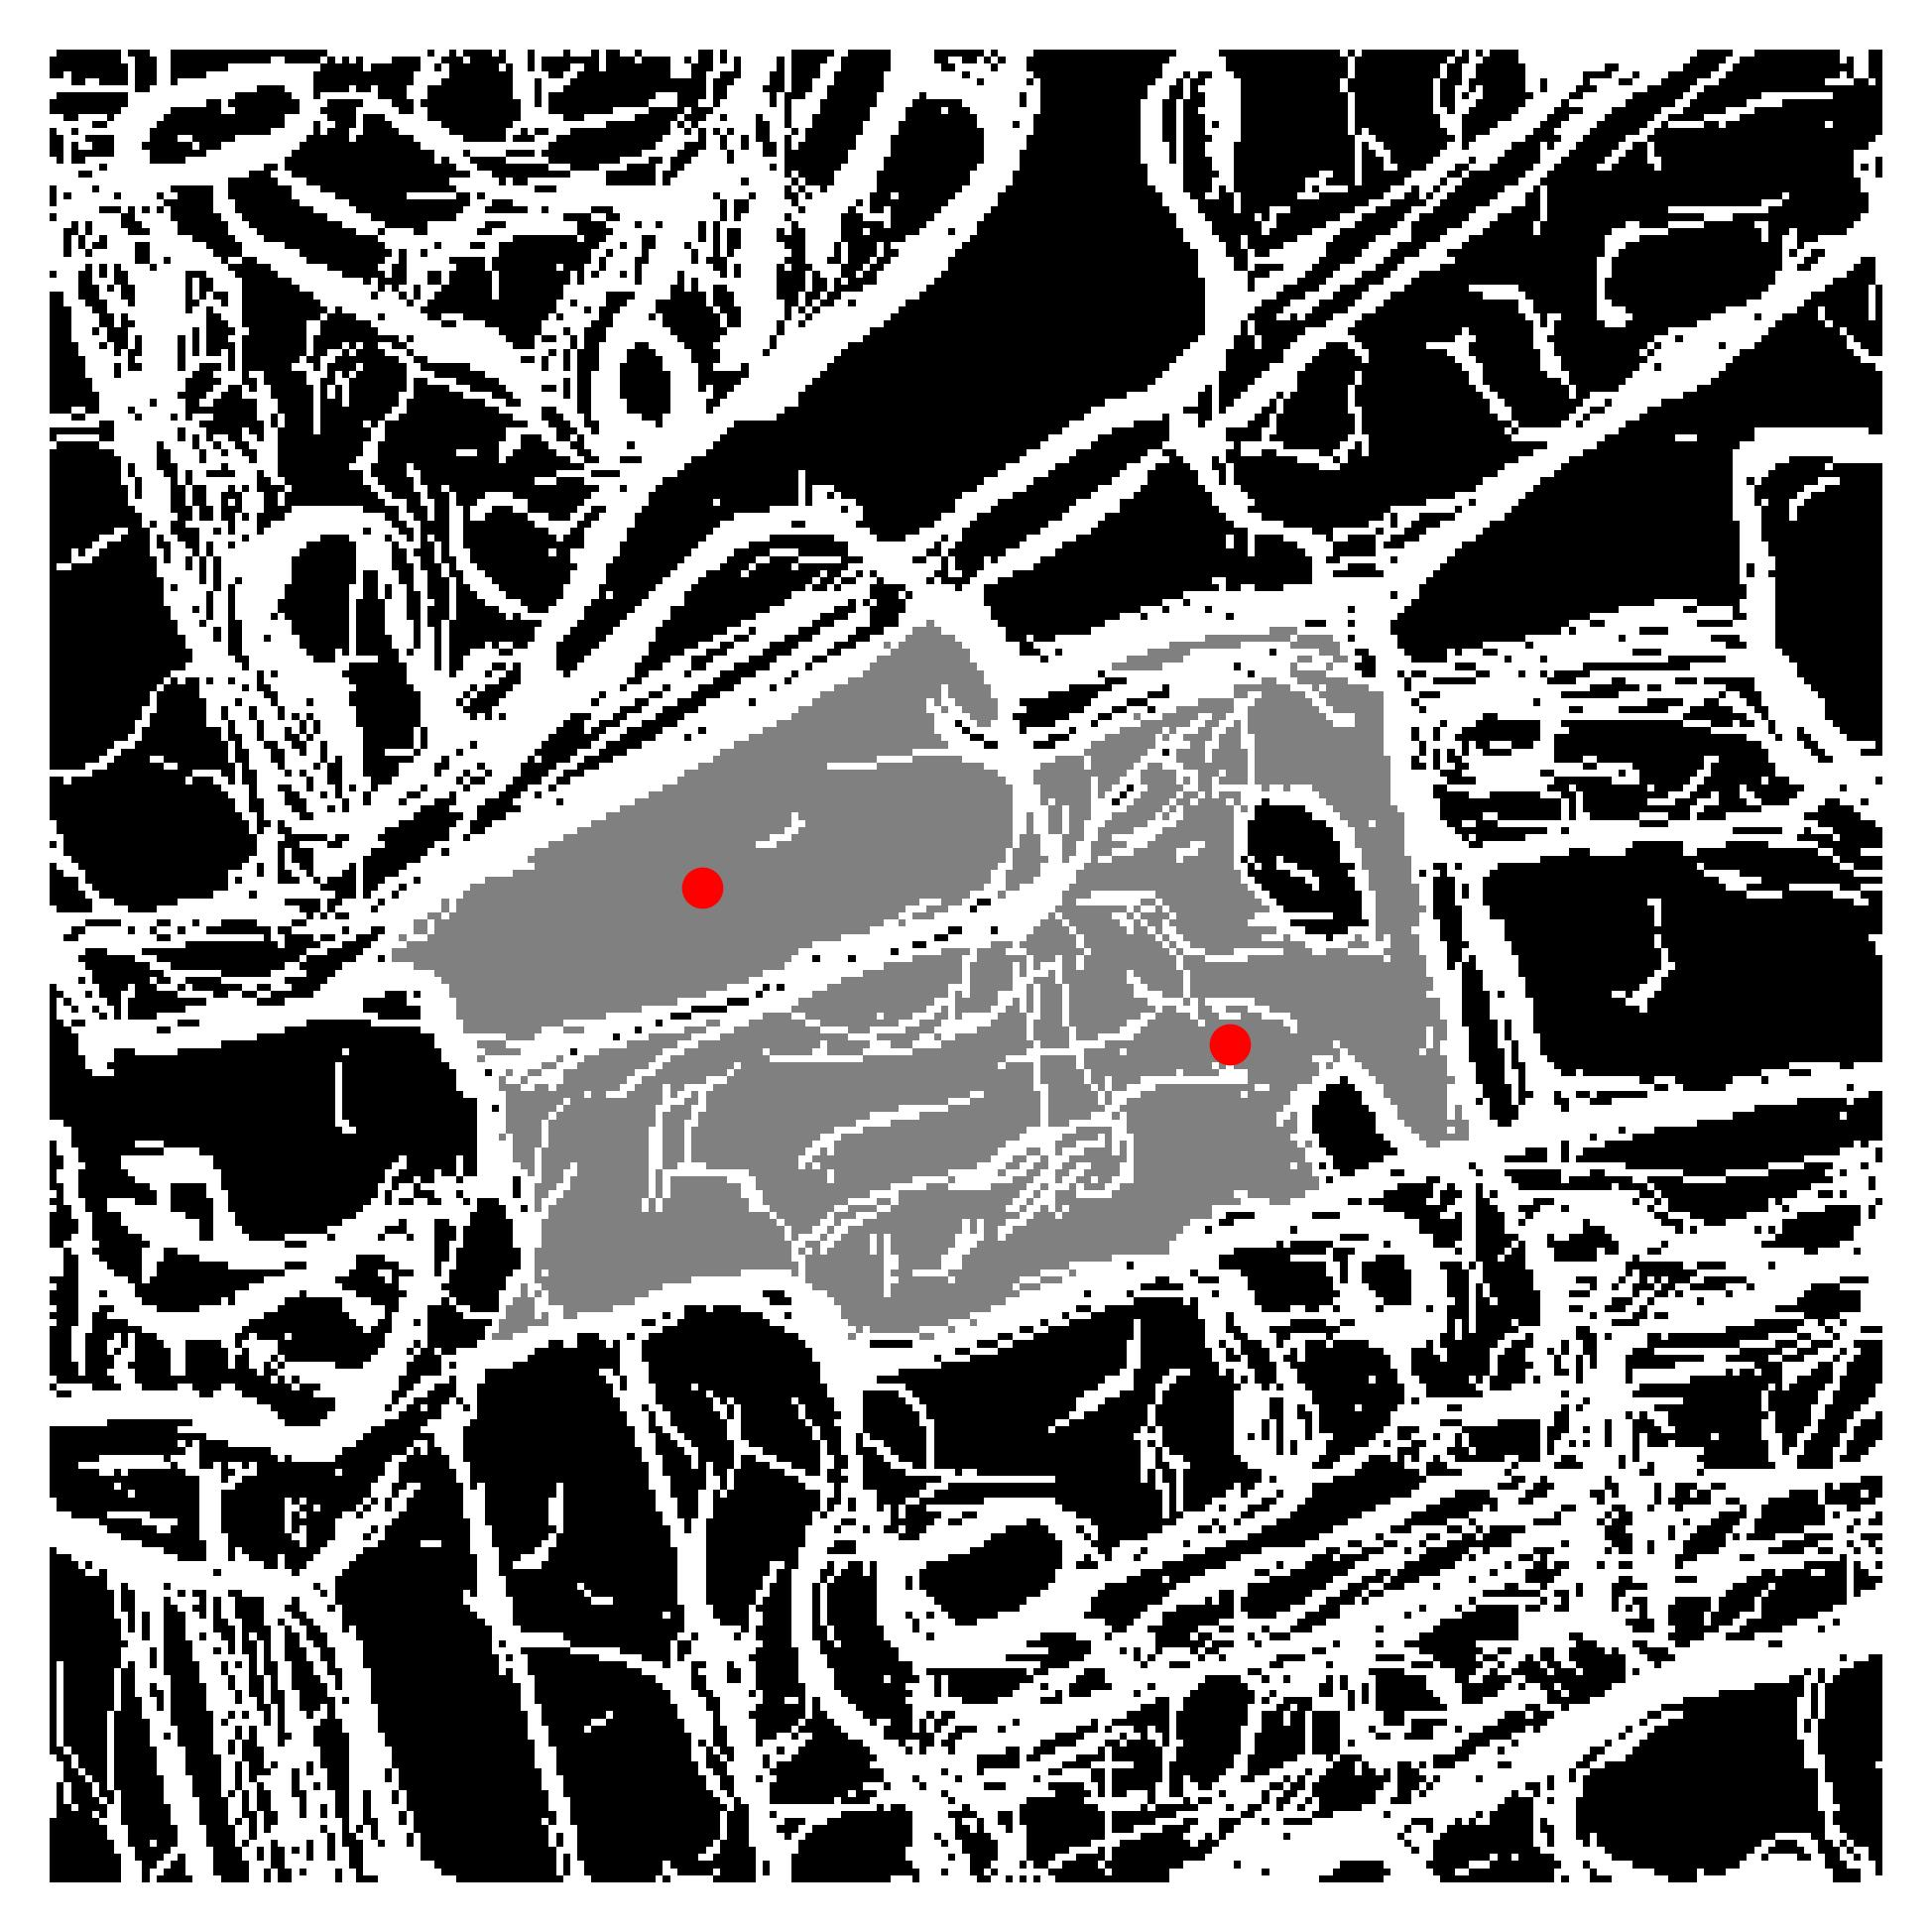
\includegraphics[width=10cm]{images/Canny1.jpg}
    \caption{Wynik uzyskany algorytmem flood fill dla dwóch punktów}
\end{figure}

Tak uzyskany obraz jest następnie przetwarzany by wyodrębnić wykryte obszary. Najpierw odbywa się progowanie z dwoma progami, które ma na celu wydobycie wypełnienia, jakie pojawiło się po poprzedniej operacji. 

\begin{figure}[H]
    \centering
    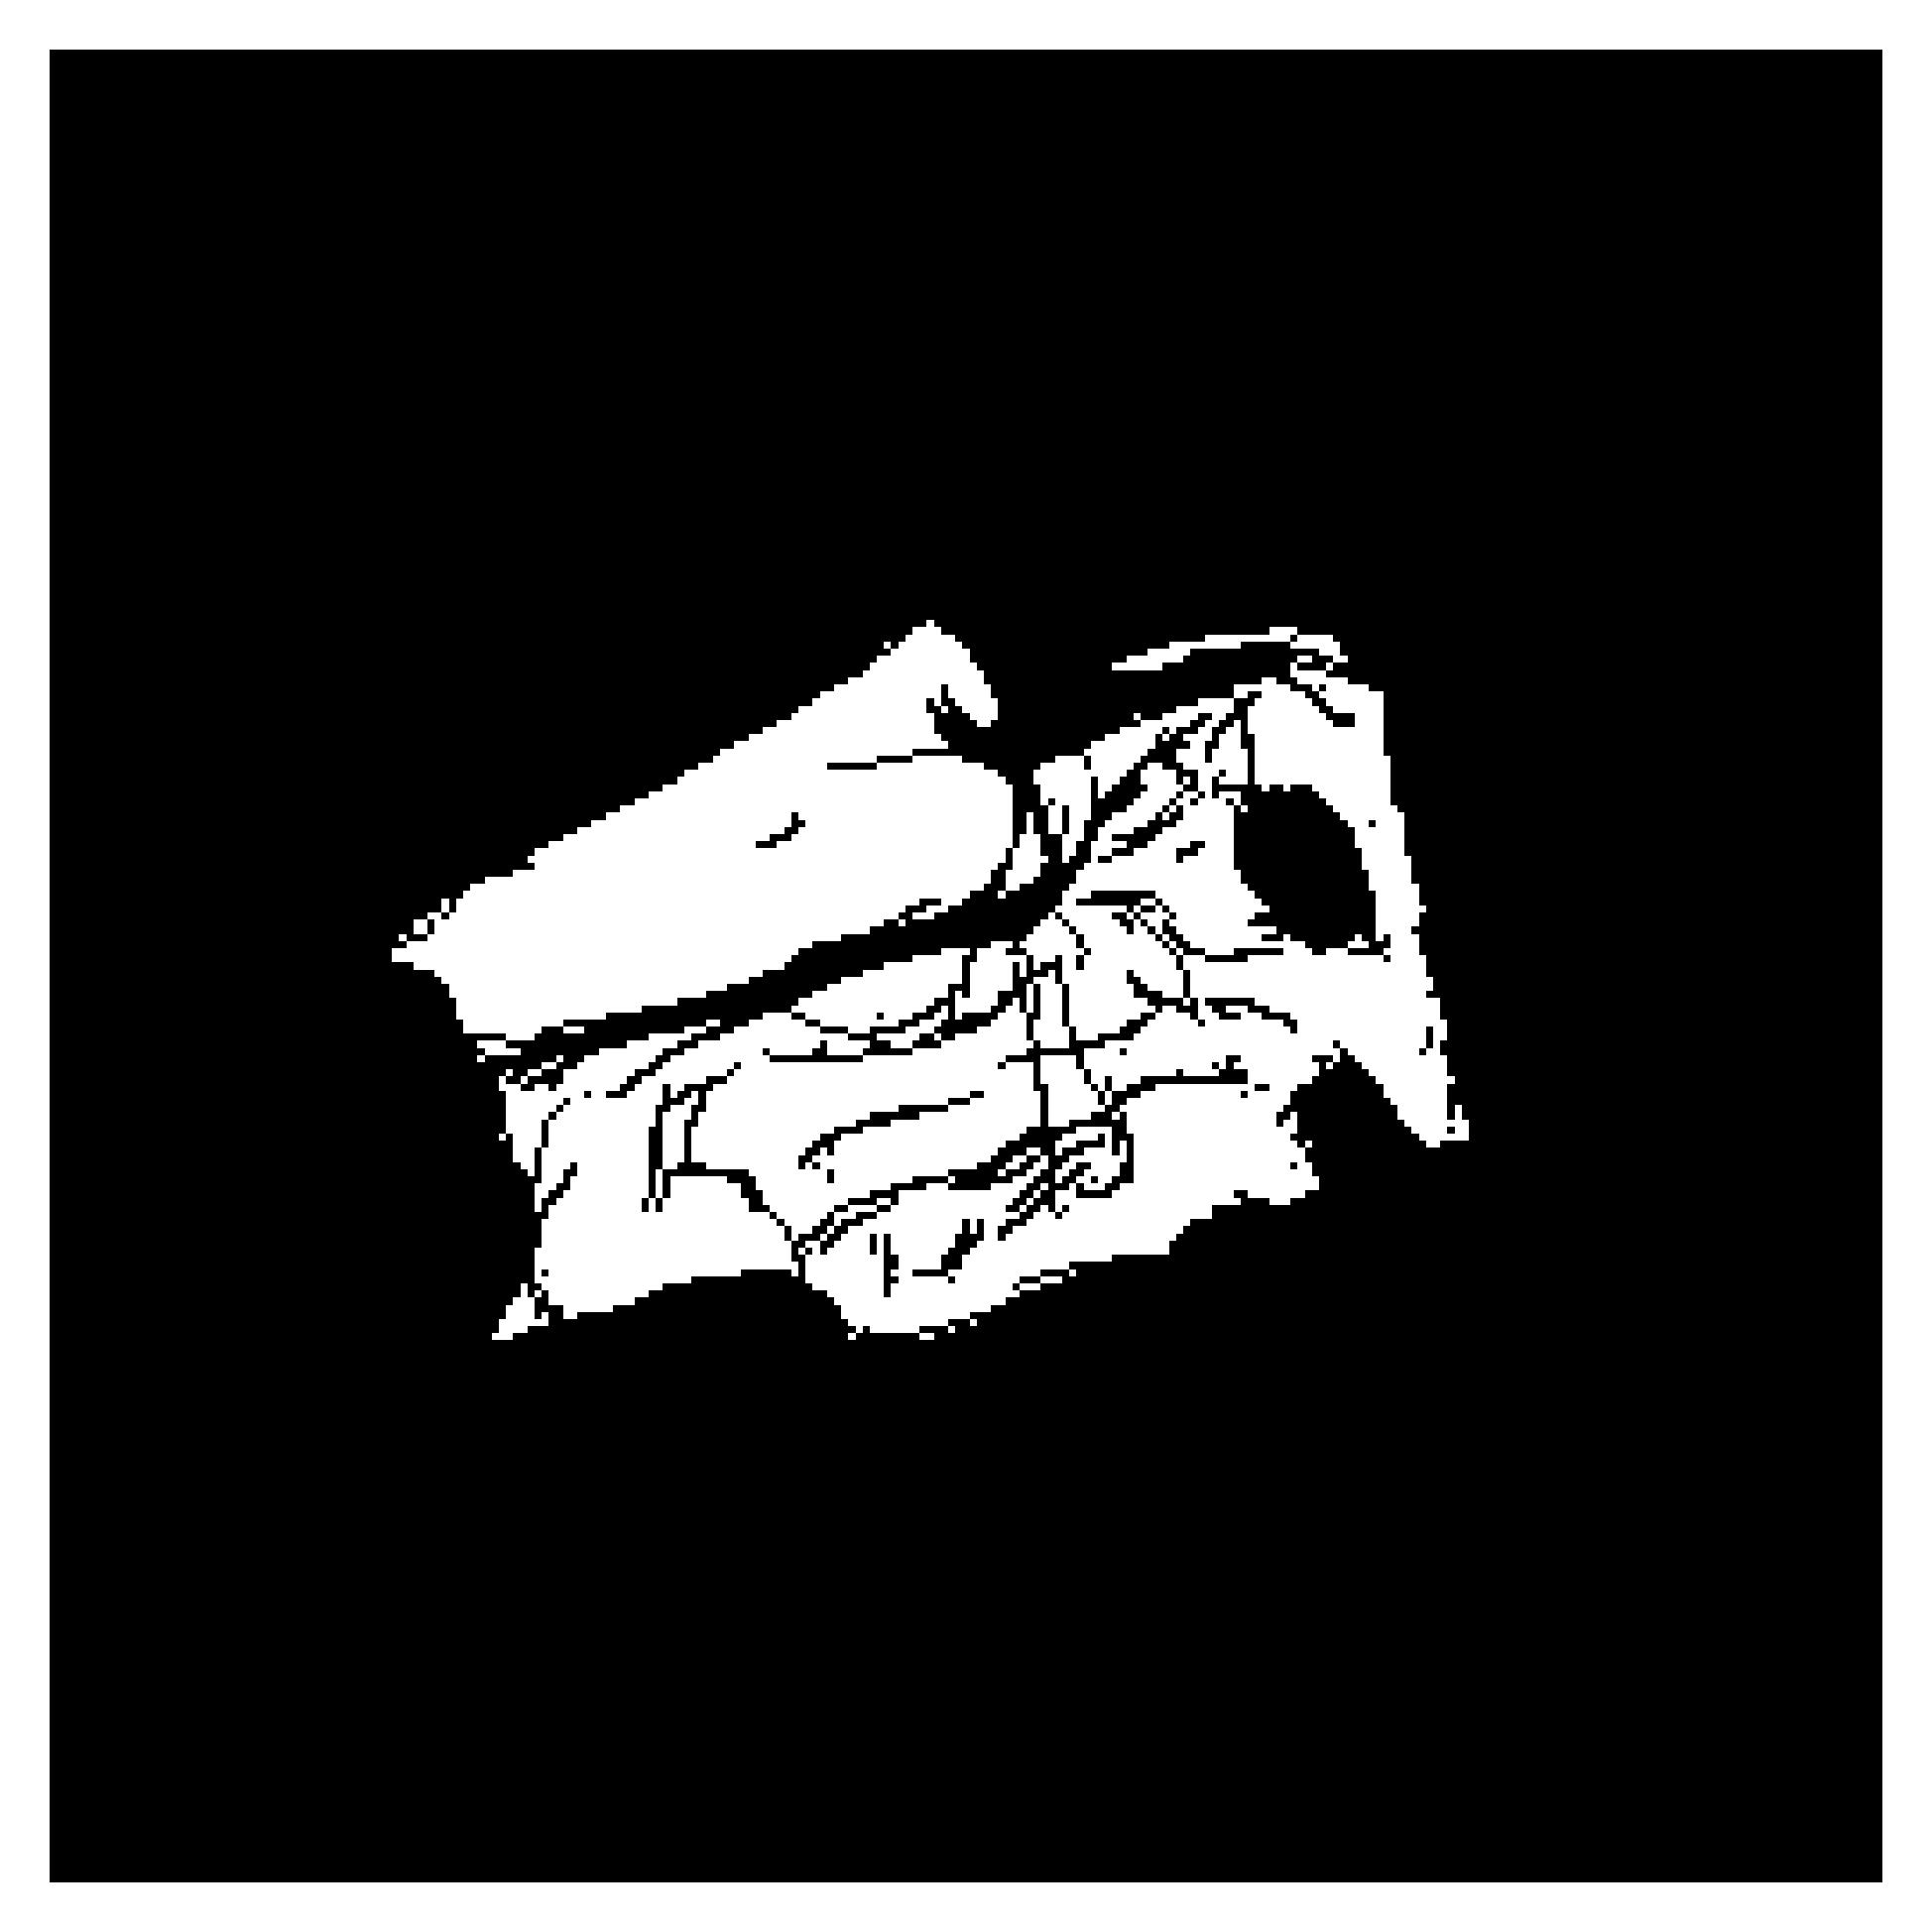
\includegraphics[width=10cm]{images/Thresholding.jpg}
    \caption{Wynik uzyskany podczas progowania}
\end{figure}

Następnie, obraz jest przetwarzany przez domknięcie morfologiczne, które pozwala na wyzbycie się nieciągłości na obrazie. 

\begin{figure}[H]
    \centering
    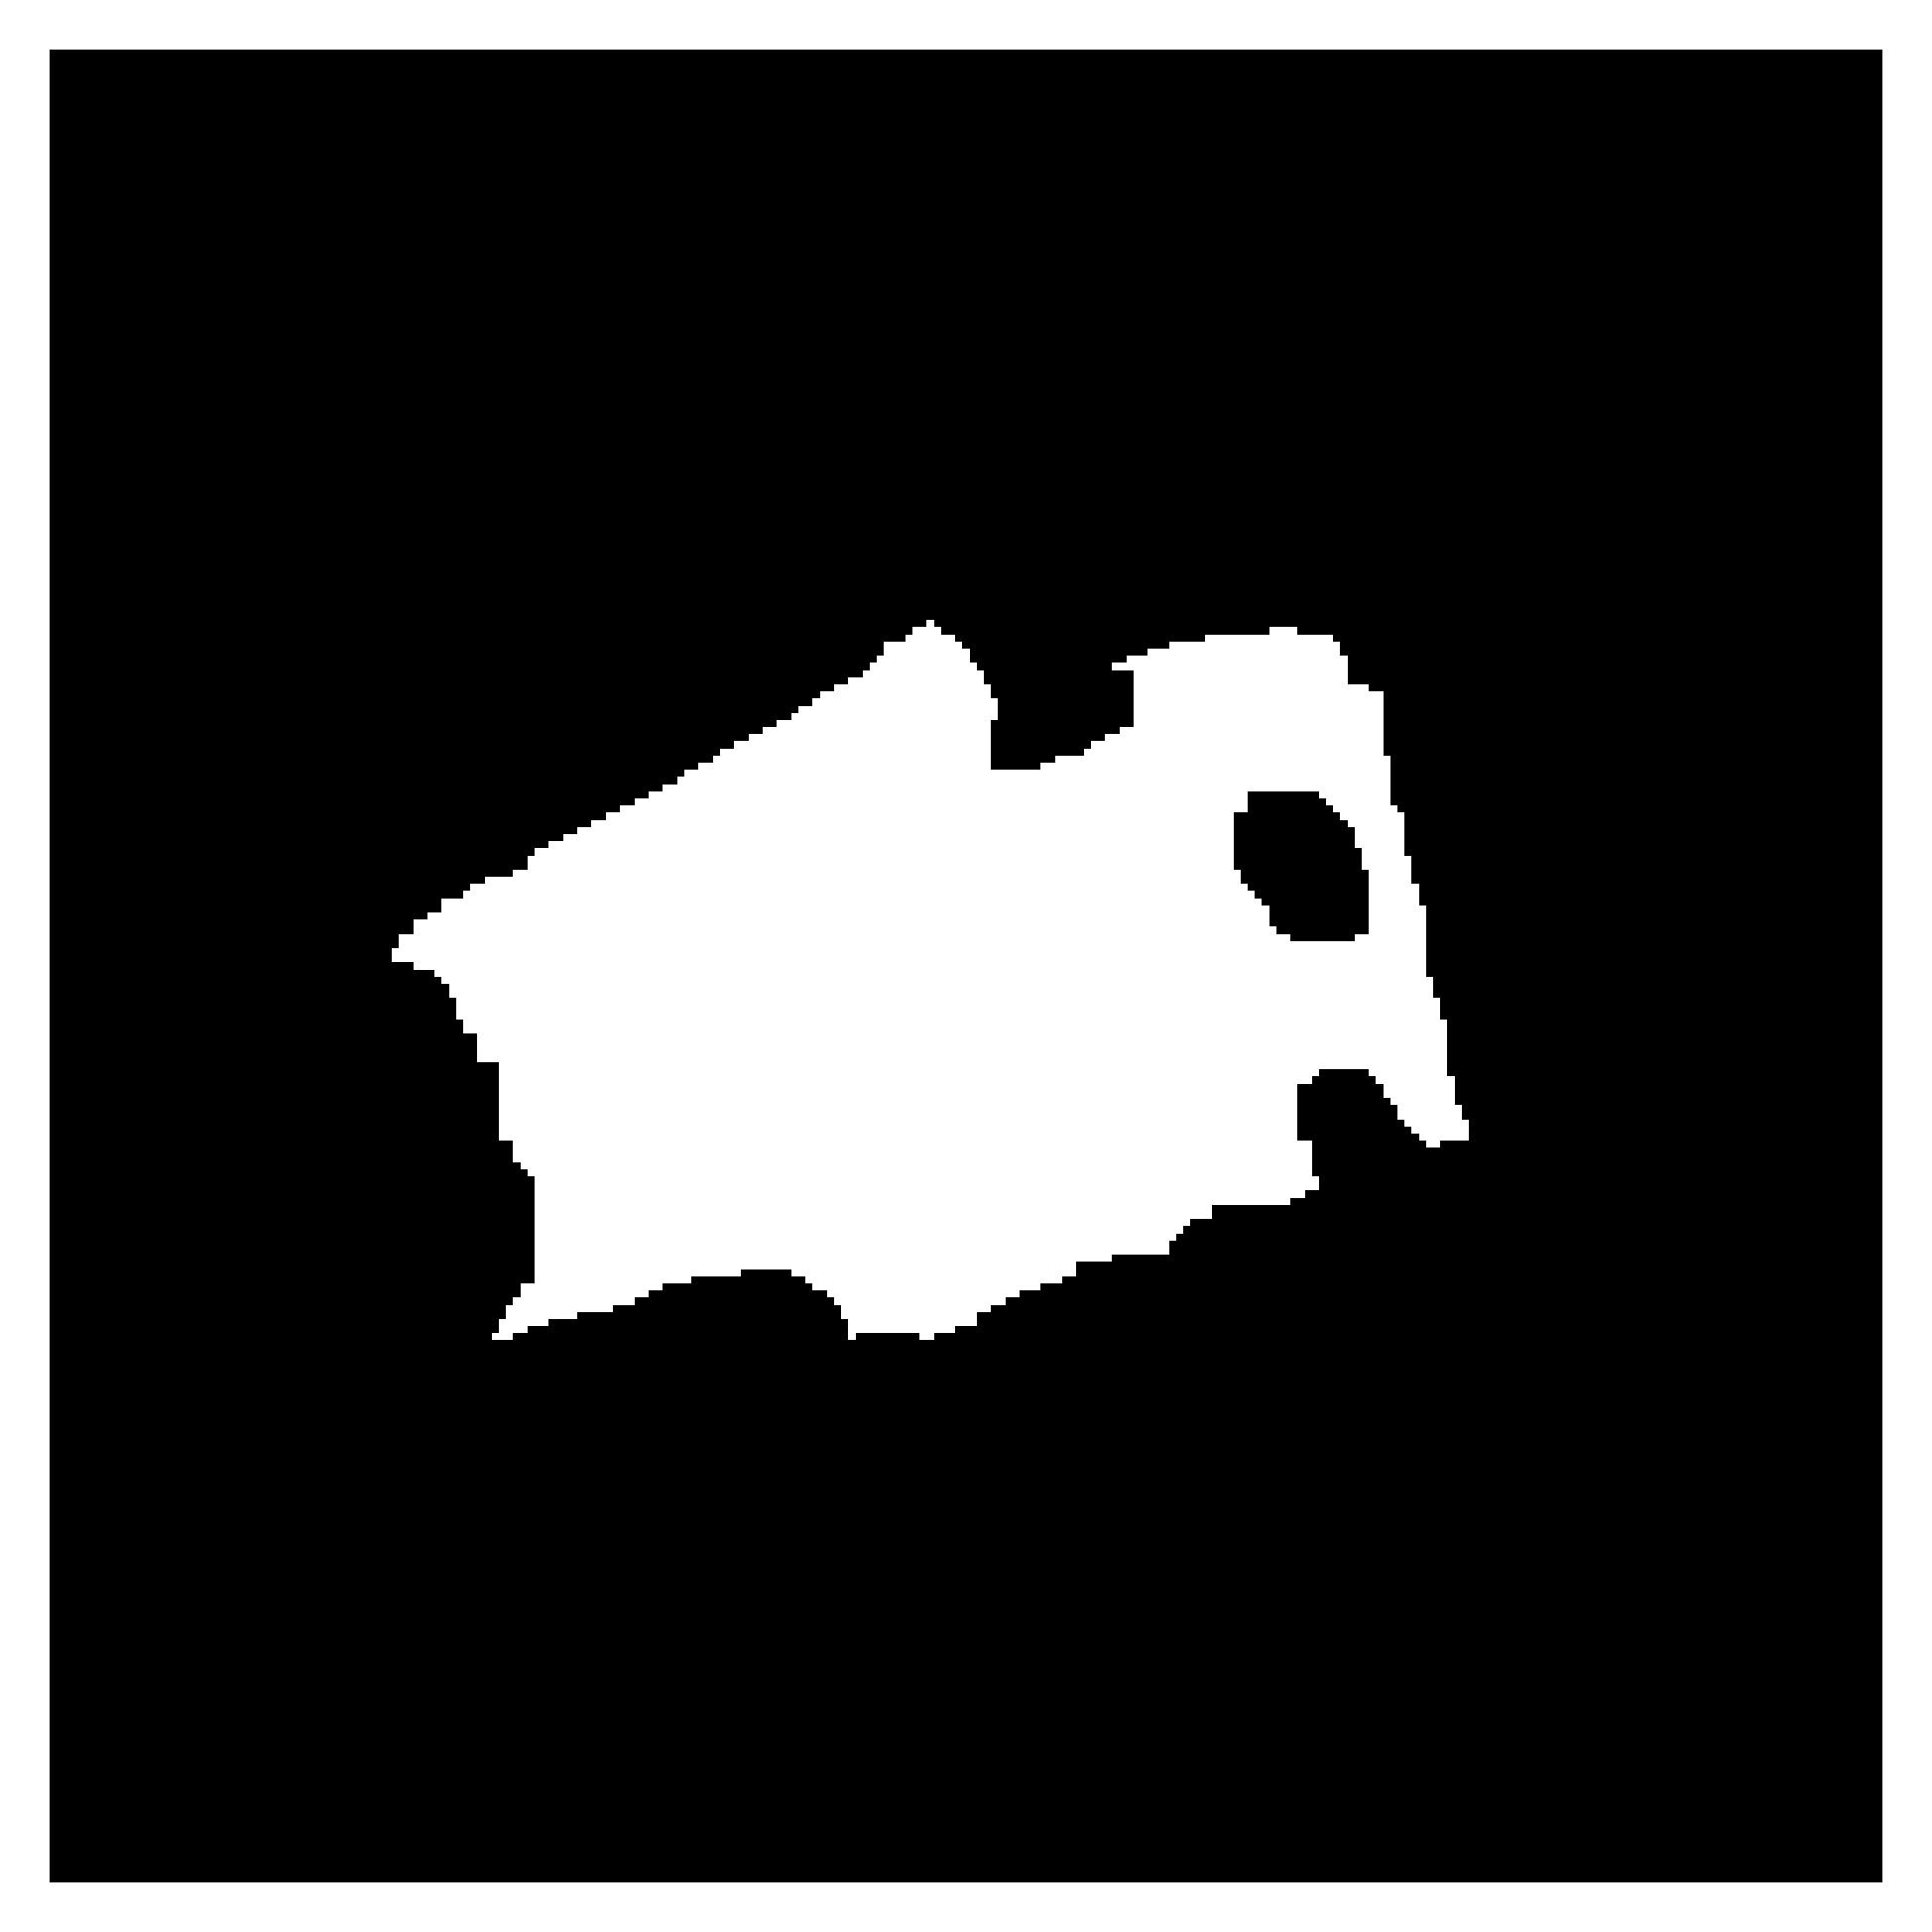
\includegraphics[width=10cm]{images/Morphology.jpg}
    \caption{Wynik uzyskany po przekształceniu morfologicznym}
\end{figure}
\newpage
Na końcu, barwy są odwracane, by przygotować obraz do wykrycia jego konturu, czego rezultatem jest lista punktów na obrazie. 

\begin{figure}[H]
    \centering
    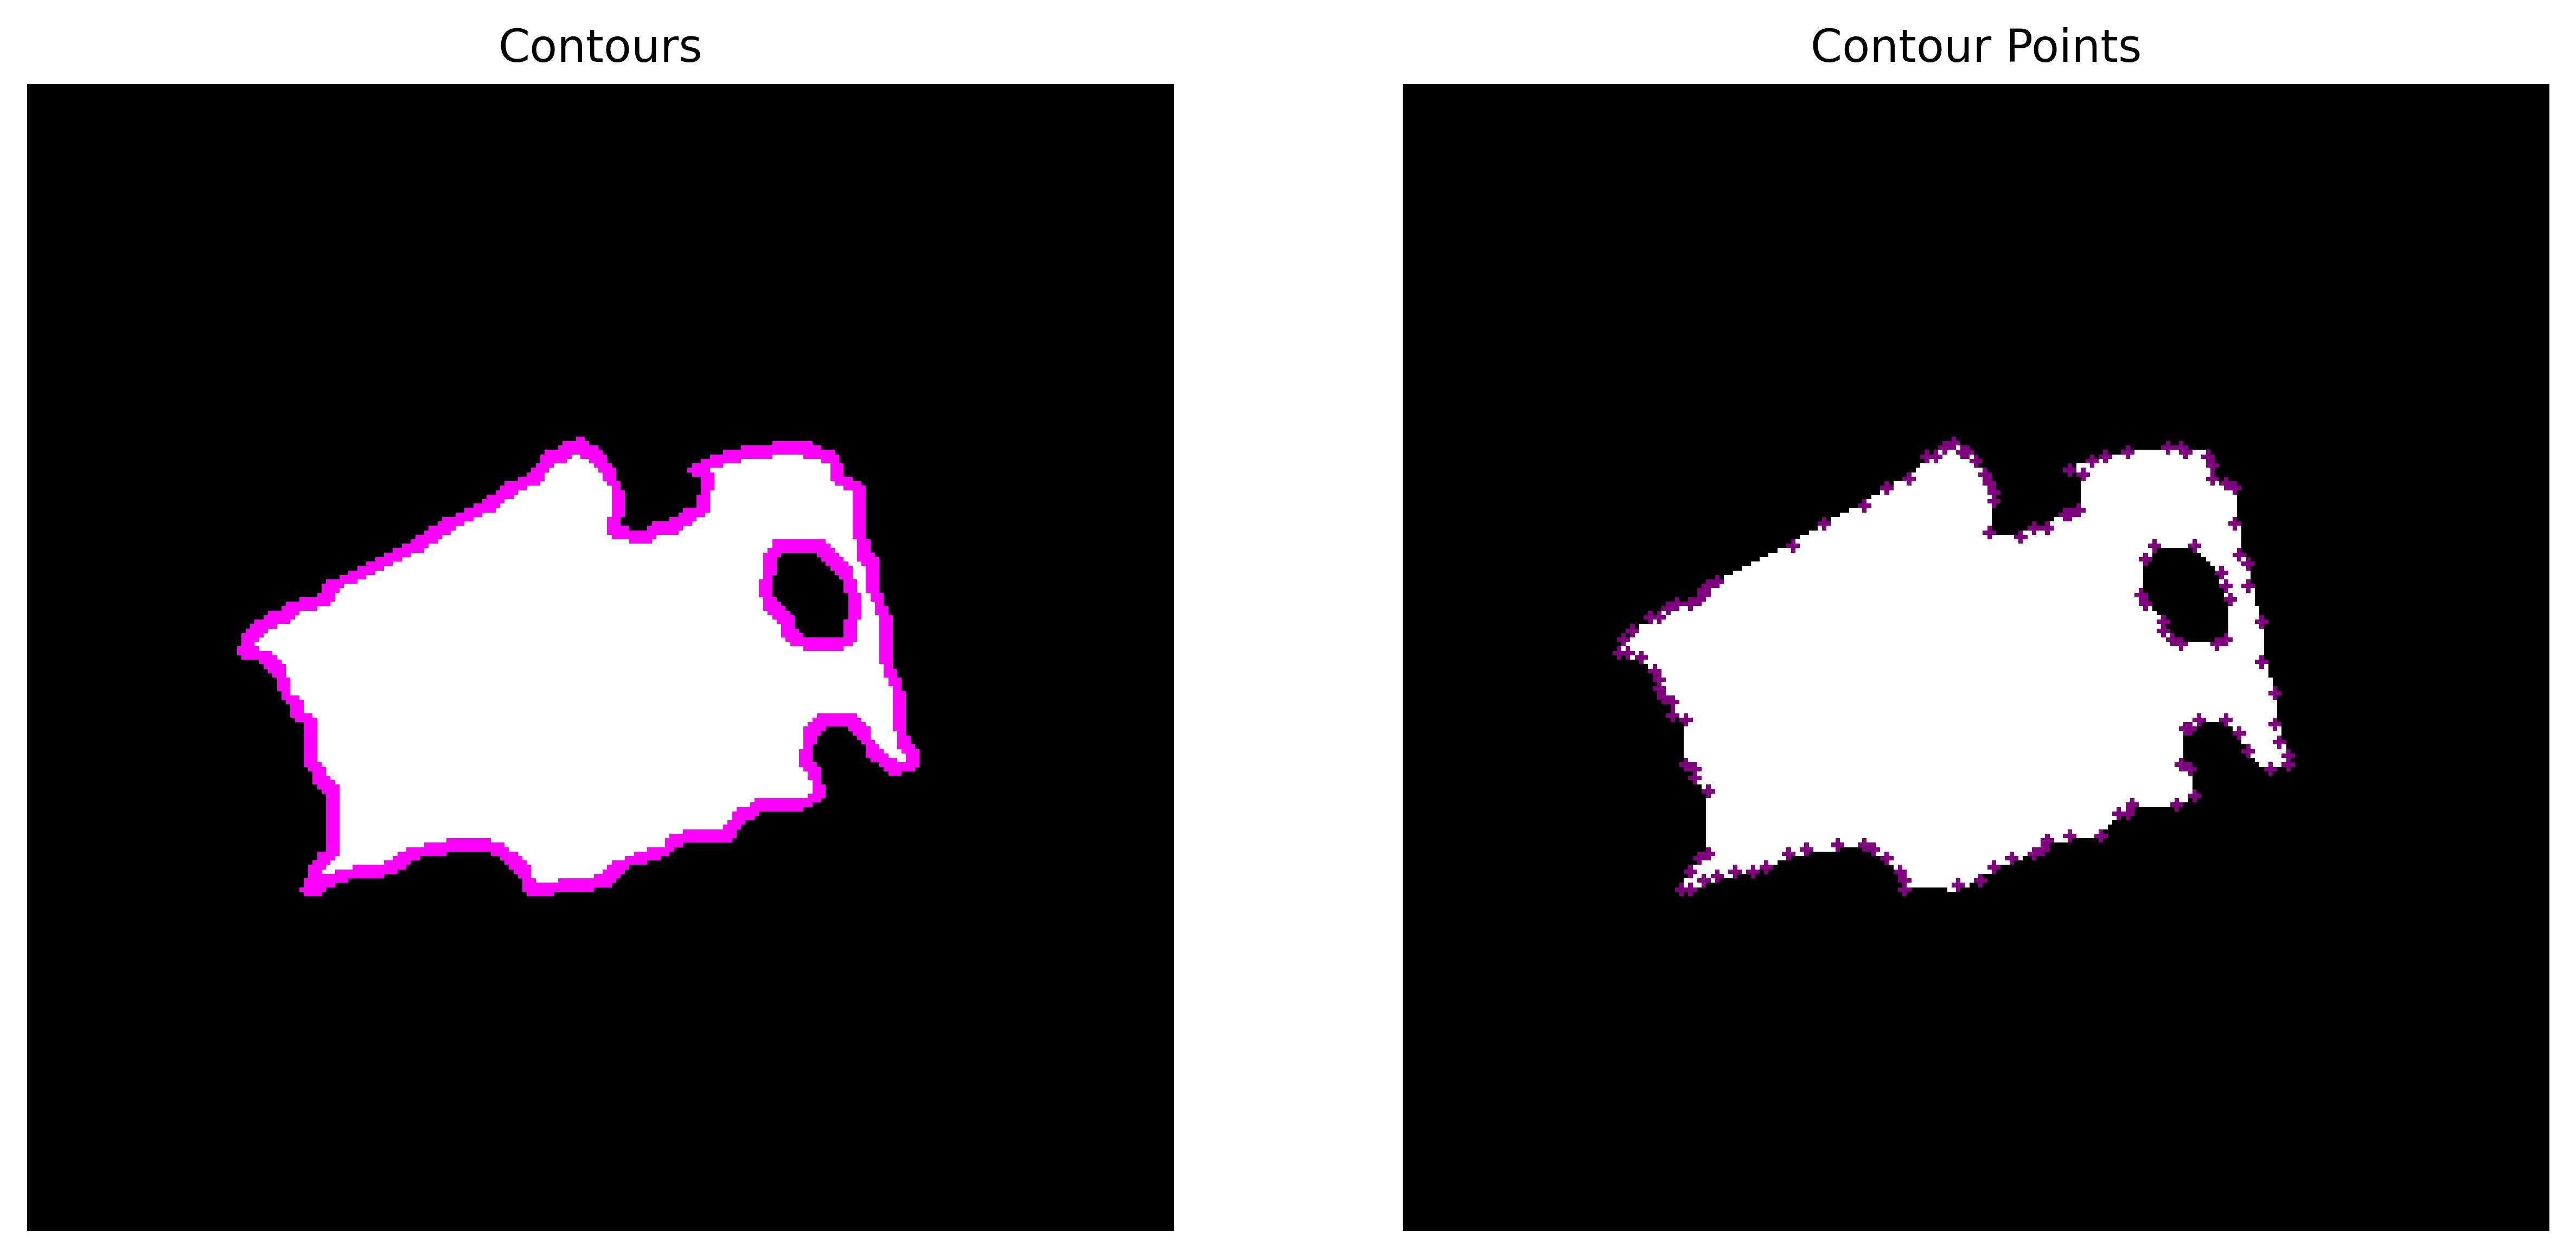
\includegraphics[width=10cm]{images/Contour.jpg}
    \caption{Kontur uzyskany w wyniku operacji na obrazie}
\end{figure}

Na powyższym obrazku widać wynik takiej operacji. Tak otrzymana lista punktów jest przeliczana na współrzędne odpowiadające tym punktom na mapie, by móc ją zwrócić do dalszego przetwarzania i wyświetlenia użytkownikowi.

\section{Planowanie trasy}

